% Indicate the main file. Must go at the beginning of the file.
% !TEX root = ../main.tex

%%%%%%%%%%%%%%%%%%%%%%%%%%%%%%%%%%%%%%%%%%%%%%%%%%%%%%%%%%%%%%%%%%%%%%%%%%%%%%%%
% 02_methods
%%%%%%%%%%%%%%%%%%%%%%%%%%%%%%%%%%%%%%%%%%%%%%%%%%%%%%%%%%%%%%%%%%%%%%%%%%%%%%%%

\section{Methods}
\label{methods}

\subsection{Data and Data Processing}%%%%%%%%%%%%%%%%%%%%%%%%%%%%%%%%%%%%%%%%%%%%%%%%%%%%

The used data for this project is at one side the SwissImage RS data from the Swiss Federal Office of Topography (swisstopo)
and on the other side a dataset generated by a team of researchers from the ZHAW concerning a ongoing project in the region of
the canton of Basel-Landschaft. The SwissImage RS data are six raster datasets with a resolution of 0.1m containing four bands: 
RGB and NIR. The dataset from the ZHAW is a feature dataset containing the landcover classification for three areas within 
the area of interest. In a first step the data was processed using ArcGIS Pro. The process included a few steps implemented as
a model \autoref{fig:processing_model}.

\begin{figure}
    \centering
    \captionsetup{width=0.8\linewidth}
    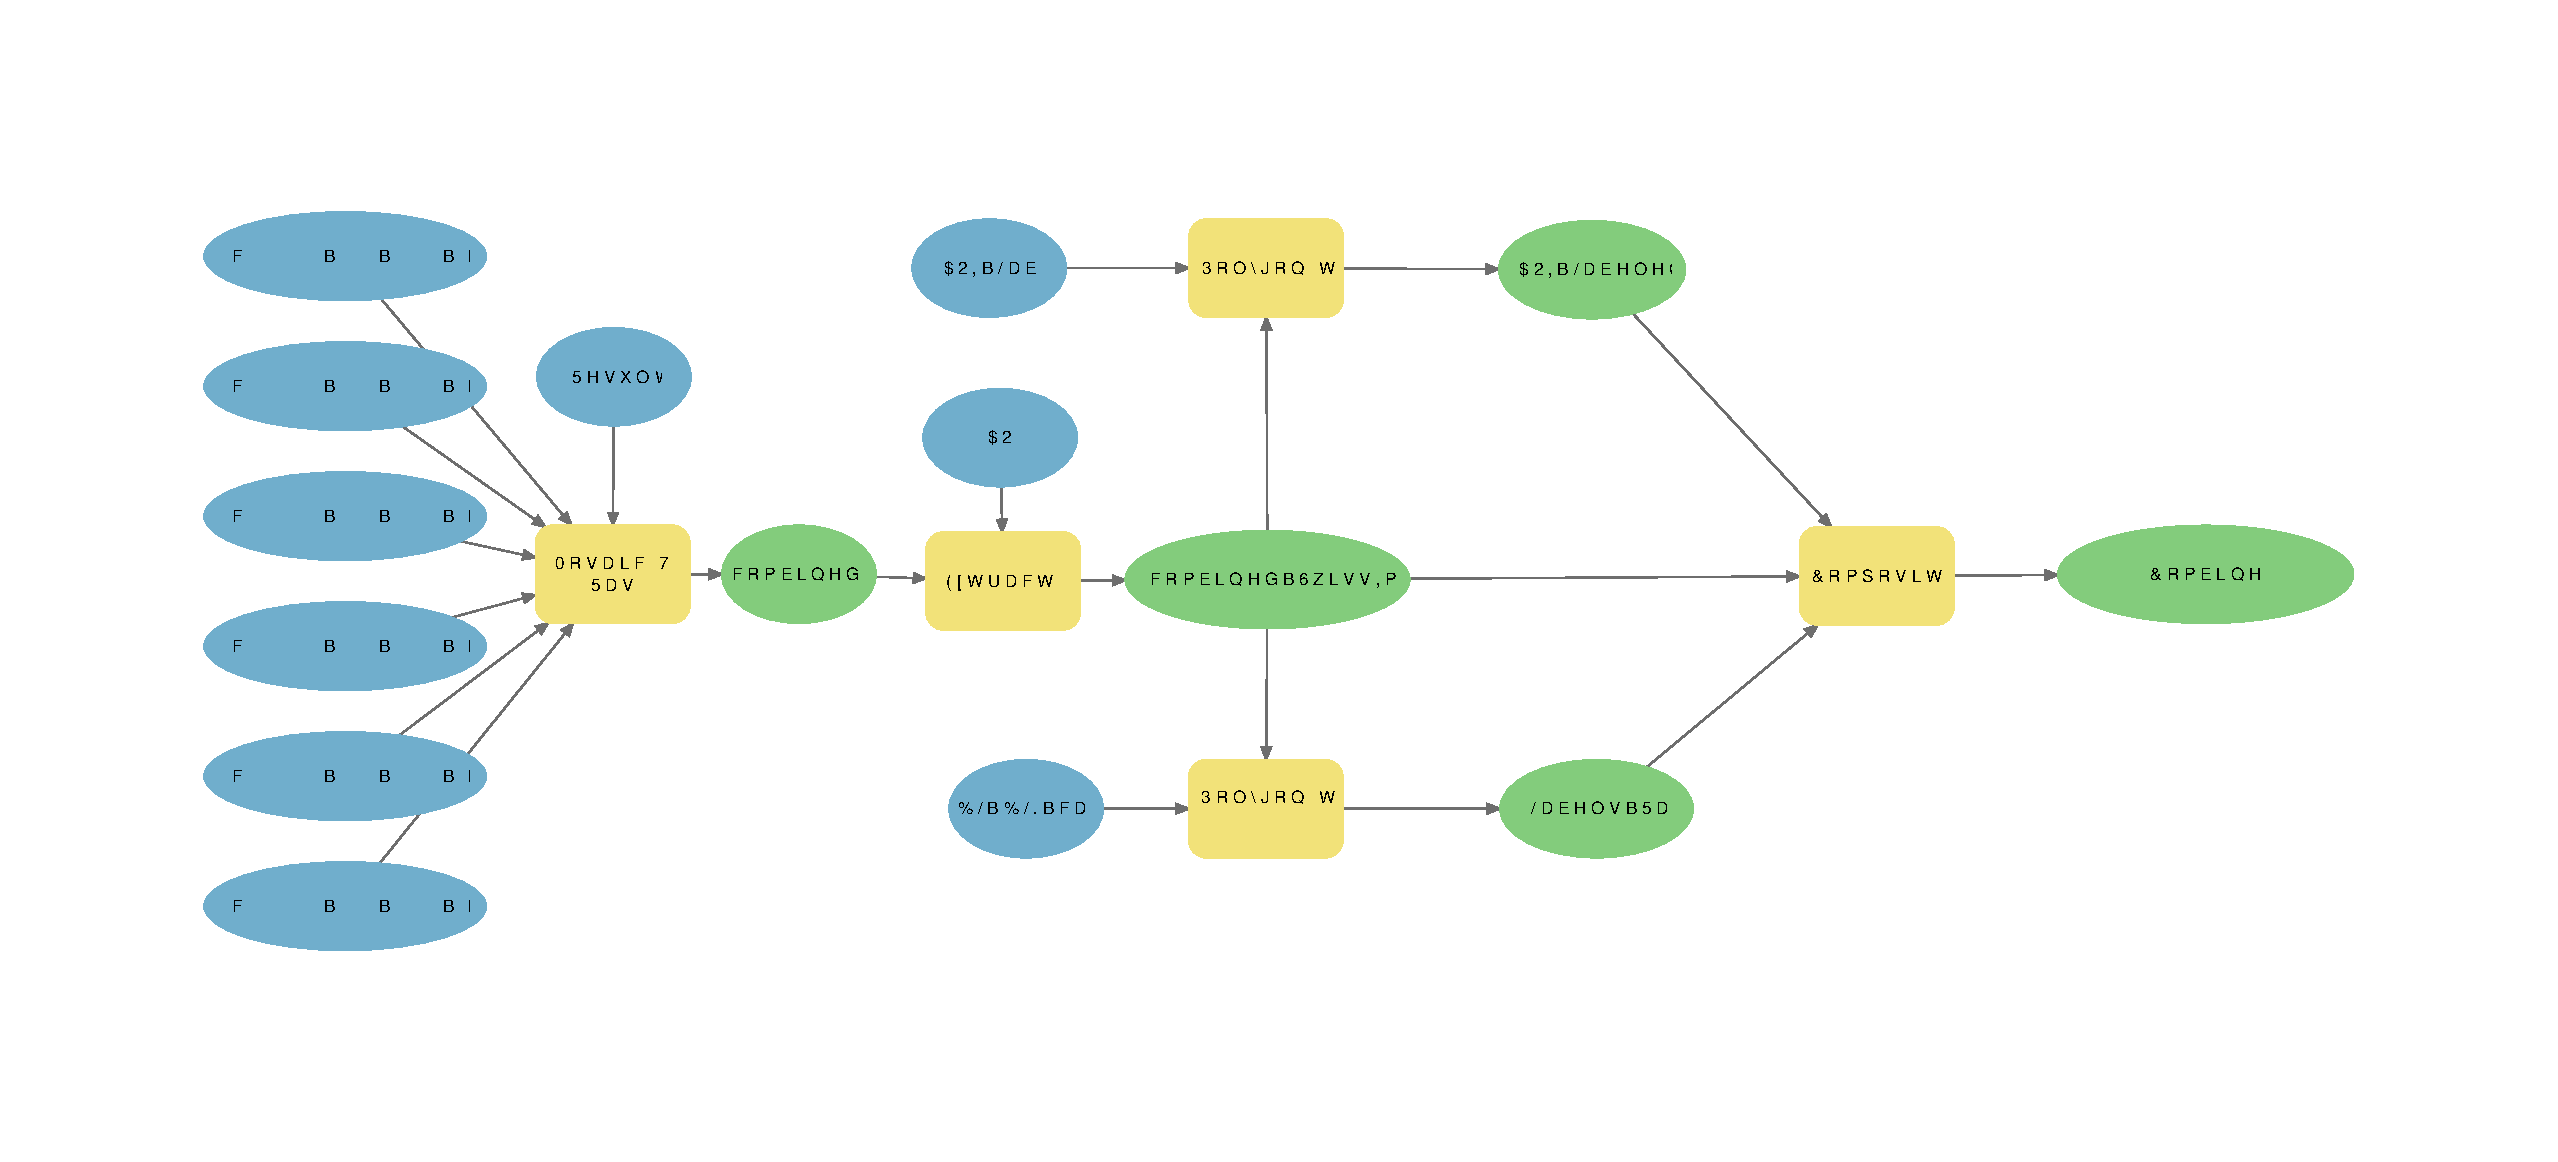
\includegraphics[width=\linewidth]{figures/Model.pdf}
    \caption{The ArcGis model used for preprocessing the data.}
    \label{fig:processing_model}
\end{figure}

\begin{figure}[H]
    \centering
    \captionsetup{width=0.8\linewidth}
    \includegraphics[scale=0.6]{figures/AOI_Labeled.png}
    \caption{The area of interest with the three labeled areas.}
    \label{fig:aoi_labeled}
\end{figure}

\begin{figure}[H]
    \centering
    \captionsetup{width=0.8\linewidth}
    \includegraphics[width=\linewidth]{figures/category_areas.png}
    \caption{The three areas with the corresponding landcover categories.}
    \label{fig:category_areas}
\end{figure}

\autoref{fig:aoi_labeled}
\autoref{fig:category_areas}